\documentclass[hyperref={pdfpagelabels=false}]{beamer}
\mode<presentation>
{
  \usetheme{Frankfurt}
  \setbeamercovered{transparent}
}
\usepackage[portuguese]{babel}
\usepackage[utf8]{inputenc} % To use characters such as é without typing é
\usepackage[absolute,overlay]{textpos} % Allows the absolute placing of text in page
\usepackage{textcomp} % provides \textrightarrow
\usepackage{ctable} % provides \toprule,\bottomrule,\midrule for tables
\let\Tiny=\tiny % eliminates compilation errors

% Basic definitions

\newcommand{\eqdef}{\stackrel{\rm def}{=}}
\newcommand{\norm}[1]{\lVert#1\rVert}
\newcommand{\fcbox}[2]{\fcolorbox{black}{#1}{\scriptsize #2}}
\newcommand{\cfcbox}[2]{\begin{center}
                        \fcolorbox{black}{#1}{\scriptsize #2}
                        \end{center}}
\definecolor{ltblue}{rgb}{0.59,0.92,0.90}
\definecolor{ltgreen}{rgb}{0.60,0.94,0.57}
\definecolor{ltrose}{rgb}{0.98,0.9,0.91}
\newcommand{\red}[1]{\textcolor{red}{#1}}
\newcommand{\blue}[1]{\textcolor{blue}{#1}}

\title{Laboratório de Matemática Computacional I} \author[M. Weber Mendonça]
{\hspace{-0.3cm}Melissa Weber Mendonça\inst{1}}
\institute[UFSC]{\inst{1} Universidade Federal de Santa Catarina} 
\date{2011}

\logo{
\includegraphics[height=1.5cm]{../../brasao_UFSC.png}}

\begin{document}
%%%
% Slide 1
\begin{frame}
% Title
  \titlepage
\end{frame}
%%%
% Slide 2
%\begin{frame}
%  \frametitle{Outline}
%  \tableofcontents[pausesections]
%\end{frame}
%%%
%
\begin{frame}
	\frametitle{Por que estudar programação?}
	\begin{block}{Objetivo}
		Entender um problema e formular sua solução usando ferramentas computacionais
	\end{block}
	\begin{block}{Ferramentas}
		Linguagem de programação MATLAB
	\end{block}
	\begin{center}
	   \begin{alertblock}{}
			\begin{center}
				Que tipo de problemas queremos resolver?
			\end{center}
	   \end{alertblock}
	\end{center}
\end{frame}
\begin{frame}
   \frametitle{Exemplos de problemas a serem resolvidos I}
   Tomografia computadorizada: \\
   
   tomo = fatia. Analisar fatias 2D de objetos 3D.
   
   $f(x)$ é o coeficiente de absorção dos raios X emitidos pela máquina no ponto $x$ do objeto; então g(L) mede os raios X (L) no lado oposto do objeto. Assim, o problema é encontrar $f(x)$ onde 
   \begin{equation*}
      g(L) = \int_L \! f(x) \, dx.
   \end{equation*}
	\begin{columns}
	   \column{5cm}{
	   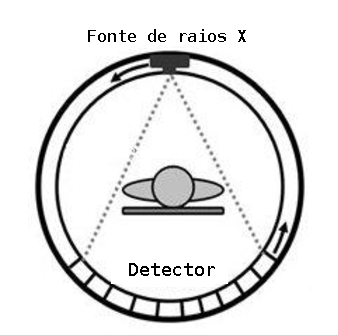
\includegraphics[width=4cm]{img/tomografia.pdf}}
	   \column{5cm}{
	   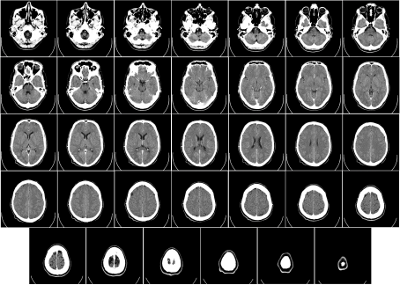
\includegraphics[width=4cm]{img/tomografia_2.png}}
	\end{columns}
\end{frame}
%
\begin{frame}
   \frametitle{Exemplos de problemas a serem resolvidos II}
   Modelagem computacional de previsão do tempo (Assimilação de Dados)
% 
	Ciclos de análise: em cada ciclo, as observações sobre o estado atual (e anterior) do sistema são combinados com os resultados de um modelo numérico de previsão do tempo, gerando uma estimativa ao estado atual do sistema (chamada de \emph{análise}. Uma vez que novas observações são feitas, o modelo é atualizado e uma nova previsão (análise futura) pode ser feita a partir do estado atual.
	
	Geração da análise:
	\begin{equation*}
	   \min_x \, \left\{ (x-x_b)^T B^{-1} (x-x_b) + (y-H(x))^TR^{-1}(y-H(x)) \right\}
	\end{equation*}

\end{frame}
%
\begin{frame}
   \frametitle{Como funciona o computador?}
   O computador é uma máquina programável que recebe uma entrada (\emph{input}), armazena e manipula automaticamente dados, e gera uma saída (\emph{output}).
   \begin{center}
		\begin{alertblock}{}
			Um computador executa funções com entrada e saída:
			\begin{center}
				entrada $\rightarrow$ ação $\rightarrow$ saída
			\end{center}
		\end{alertblock}
	\end{center}
\end{frame}
%
\begin{frame}
   \frametitle{Primeiros "computadores"}
   Em 1613, a palavra "computador" aparece pela primeira vez, designando uma pessoa que realizasse cálculos.
   
   Os computadores antigos não eram máquinas programáveis, mas serviam a uma função específica. 
   
   Exemplos: ábaco, régua de cálculo, astrolábio, calculadora.
   \begin{columns}
      \column{2cm}
      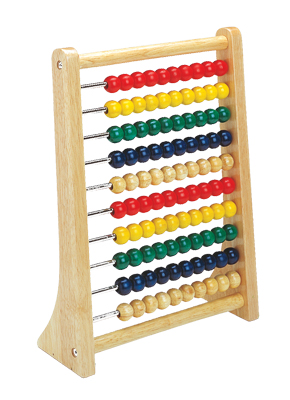
\includegraphics[width=2cm]{img/abaco.jpg}
      \column{2cm}
      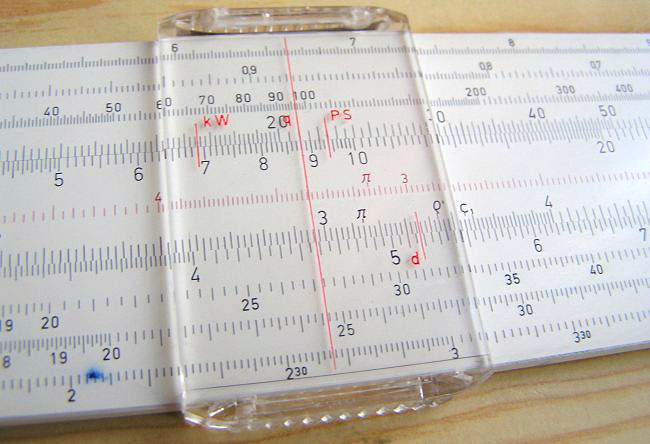
\includegraphics[width=2cm]{img/regua_de_calculo.jpg}
      \column{2cm}
      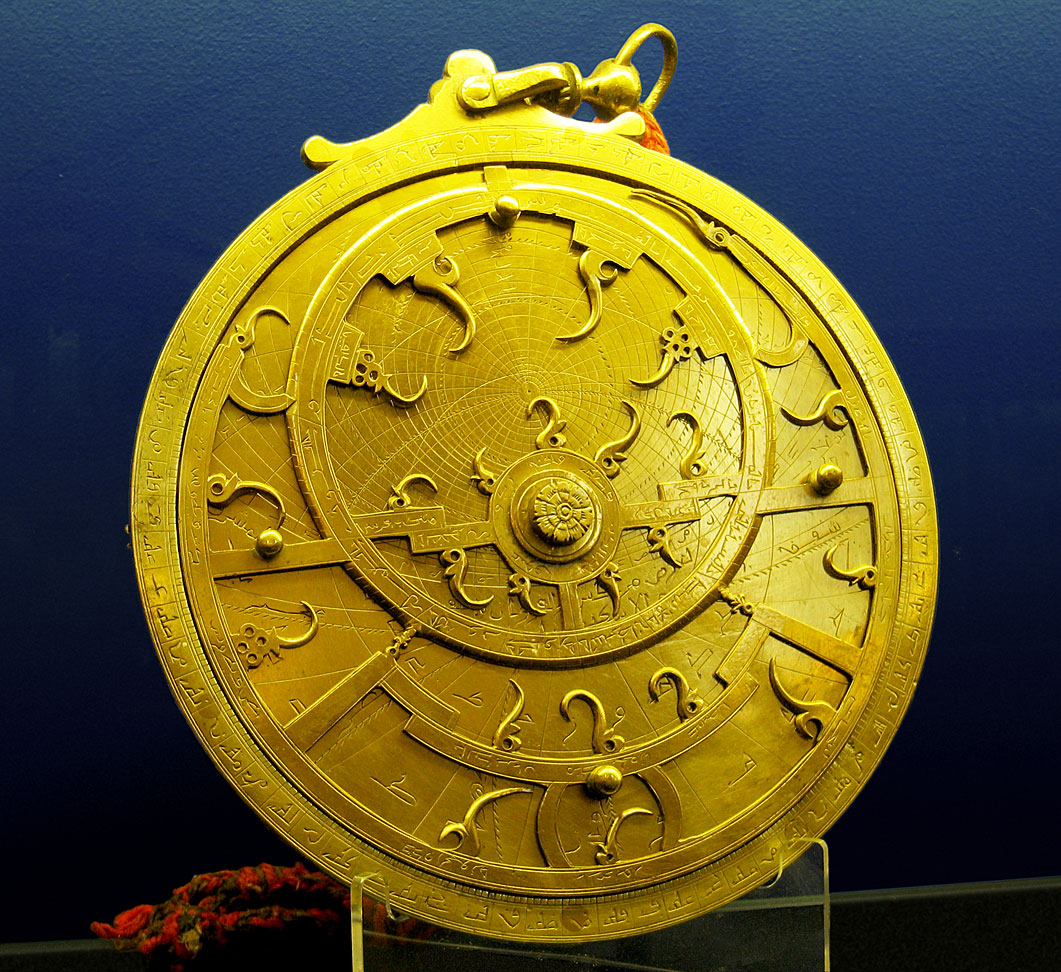
\includegraphics[width=2cm]{img/astrolabio.jpg}
      \column{2cm}
      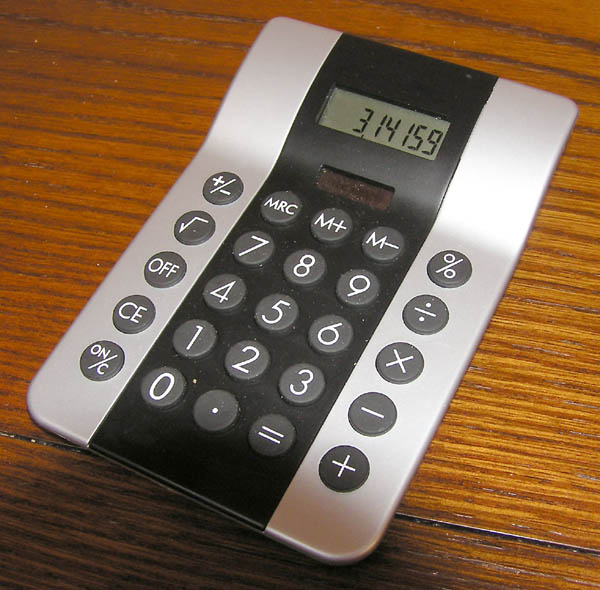
\includegraphics[width=2cm]{img/calculadora.jpg}
   \end{columns}
\end{frame}
%
\begin{frame}
   \frametitle{Computadores programáveis de uso limitado}
   Em 1801, Joseph Marie Jacquard introduziu o uso de cartões perfurados para programar um tear e produzir padrões intrincados de tecido automaticamente.
   \vspace{0.4cm}
   \begin{center}
   \begin{columns}
      \column{5cm}
			\begin{center}
			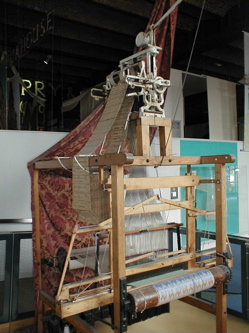
\includegraphics[height=4.5cm]{img/jacquard.jpg}
			\end{center}
      \column{5cm}
			\begin{center}
			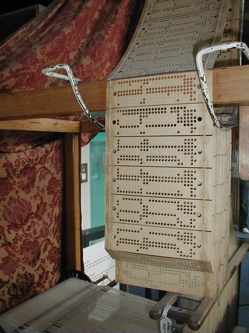
\includegraphics[height=4.5cm]{img/jacquard_cartao.jpg}
			\end{center}
   \end{columns}
   \end{center}
\end{frame}
\begin{frame}
   \frametitle{Computadores programáveis de uso geral}
   Em 1837, Charles Babbage imaginou o conceito de um computador mecânico totalmente programável (a \emph{máquina analítica}) - mas não chegou a construi-la.
   	\begin{center}
		   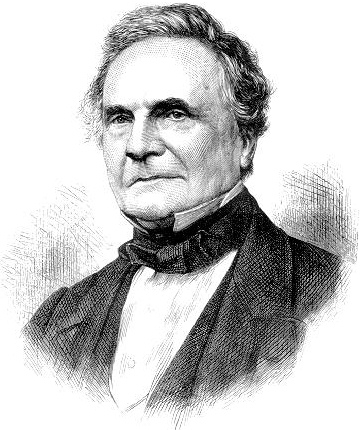
\includegraphics[height=4.5cm]{img/CharlesBabbage.jpg}
		\end{center}
\end{frame}
\begin{frame}
   \frametitle{Computadores programáveis de uso geral}
   Ada Augusta Byron King, Condessa de Lovelace, filha do poeta britânico Lord Byron, é reconhecida como a primeira programadora de toda a história. Ela desenvolveu os \emph{algoritmos} que permitiriam à máquina de Babbage computar valores de funções matemáticas, além de publicar uma coleção de notas sobre a máquina analítica.
	\begin{center}
		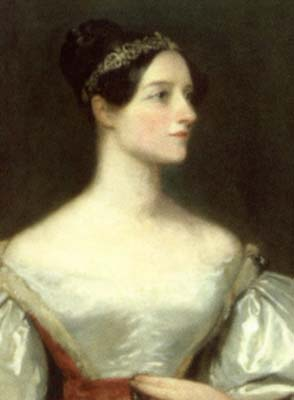
\includegraphics[height=4.5cm]{img/ada.jpeg}
	\end{center}
\end{frame}
\begin{frame}
   \frametitle{Estrutura de um computador moderno}
   \begin{center}
      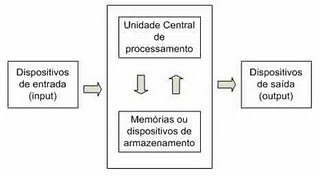
\includegraphics{img/cpu.jpg}
   \end{center}
\end{frame}
\begin{frame}
	\frametitle{O que é um algoritmo?}
   \begin{center}
      Um algoritmo é uma sequência \alert{finita} de passos que tem como objetivo realizar alguma tarefa.
   \end{center}

	Exemplo: receita de bolo.
   \begin{itemize}
		\item Entrada: ingredientes, utensílios usados.
		\item Ação: bater, misturar, picar, assar.
		\item Saída: bolo.
	\end{itemize}
\end{frame}
\begin{frame}
   \frametitle{Exemplo: Como ferver água (no fogão)?}
	\only<1->{Dada uma cozinha}\only<2->{, com uma pia com torneira e água corrente}\only<3->{, um fogão com pelo menos uma boca}\only<4->{, e uma chaleira ou panela}\only<5->{, faça o seguinte:}
   \only<5->{
   \begin{itemize}}
		\only<5>{\item }
		\only<6->{\item Se encontrar uma chaleira, então use esta chaleira. \\
					       Senão, use uma panela.}
      \only<7->{\item Levar a chaleira ou panela até a pia.}
      \only<8->{\item Encher a chaleira ou panela de água.}
      \only<9->{\item Acender uma das bocas do fogão.}
      \only<10->{\item Colocar a chaleira ou panela sobre a boca acesa do fogão.}
      \only<11->{\item Enquanto a água não estiver borbulhando, \\
							 continue aguardando.}
      \only<12->{\item Desligue a boca acesa do fogão.}
   \only<5->{
   \end{itemize}}
   \only<13->{A água está fervida dentro da chaleira ou panela.}
\end{frame}
\begin{frame}
   \frametitle{Exemplo: Como ferver água (no fogão)?}
   ENTRADA: cozinha, pia, torneira, água corrente, fogão com pelo menos uma boca, chaleira ou panela.\\
   AÇÃO: 
   \begin{itemize}
      \item Se encontrar uma chaleira, então pegue esta chaleira como recipiente. \\
				Senão, pegue uma panela como recipiente.
      \item Levar o recipiente até a pia.
      \item Encher o recipiente de água.
      \item Acender uma das bocas do fogão.
      \item Colocar o recipiente sobre a boca acesa do fogão.
      \item Enquanto a água não estiver borbulhando, \\
				continue aguardando.
      \item Desligue a boca acesa do fogão.
   \end{itemize}
	SAÍDA: recipiente com água fervida.
\end{frame}
\begin{frame}
   \frametitle{Exemplo: Como ferver água (no fogão)?}
   ENTRADA: cozinha, pia, torneira, água corrente, fogão com pelo menos uma boca, chaleira ou panela.\\
   AÇÃO: 
   \begin{itemize}
      \item \alert{Se} encontrar uma chaleira, então pegue esta chaleira como recipiente. \\
				\alert{Senão}, pegue uma panela como recipiente.
      \item Levar o recipiente até a pia.
      \item Encher o recipiente de água.
      \item Acender uma das bocas do fogão.
      \item Colocar o recipiente sobre a boca acesa do fogão.
      \item \alert{Enquanto} a água não estiver borbulhando, \\
				\alert{continue} aguardando.
      \item Desligue a boca acesa do fogão.
   \end{itemize}
	SAÍDA: recipiente com água fervida.
\end{frame}
\begin{frame}
   \frametitle{Exemplo: Como ferver água (no fogão)?}
   ENTRADA: cozinha, pia, torneira, água corrente, fogão com pelo menos uma boca, chaleira ou panela.\\
   AÇÃO: 
   \begin{itemize}
		\item Se encontrar uma chaleira, então pegue esta chaleira como \blue{recipiente}. \\
		      Senão, pegue uma panela como \blue{recipiente}.
      \item Levar o \blue{recipiente} até a pia.
      \item Encher o \blue{recipiente} de água.
      \item Acender uma das bocas do fogão.
      \item Colocar o \blue{recipiente} sobre a boca acesa do fogão.
      \item Enquanto a água não estiver borbulhando, \\
			   continue aguardando.
      \item Desligue a boca acesa do fogão.
   \end{itemize}
   SAÍDA: recipiente com água fervida.
\end{frame}
%
\begin{frame}
   \frametitle{Exemplo: Como ferver água (no fogão)?}
   ENTRADA: cozinha, pia, torneira, água corrente, fogão com pelo menos uma boca, chaleira ou panela.\\
   AÇÃO: 
   \begin{itemize}
      \item Se existe chaleira, então recipiente \only<1>{\alert{$\leftarrow$}}\only<2>{$\leftarrow$} chaleira. \\
				Senão, recipiente \only<1>{\alert{$\leftarrow$}}\only<2>{$\leftarrow$} panela.
      \item Levar o recipiente até a pia.
      \item Encher o recipiente de água.
      \item \only<1>{Acender uma das bocas do fogão.}
            \only<2>{\alert{Acender} uma das bocas do fogão.}
      \item Colocar o recipiente sobre a boca acesa do fogão.
      \item Enquanto a água não estiver borbulhando, \\
				continue aguardando.
      \item Desligue a boca acesa do fogão.
   \end{itemize}
   SAÍDA: recipiente com água fervida.
\end{frame}
%
\begin{frame}
	\frametitle{O que é uma linguagem de programação?}
	Uma linguagem de programação traduz um algoritmo (sequência de instruções) da linguagem humana para a linguagem da máquina ("0 e 1").
	
	Existem milhares de linguagens de programação.
\end{frame}
%
\begin{frame}
   \frametitle{Módulo: Exemplo em Pseudo-código}
   \begin{center}
	\begin{itemize}
		\item[] Dado um número $a$
		\item[]
		\item[] Se $a > 0$, então
		\begin{itemize}
		   \item[] módulo $= a $
		\end{itemize}
		\item[] Senão
		\begin{itemize}
		   \item[] módulo $= -a$
		\end{itemize}
		\item[] Fim Se
	\end{itemize}
	\end{center}
\end{frame}
\begin{frame}
   \frametitle{Exemplo em Python}
   \begin{center}
	\begin{itemize}
		\item[] def modulo(a):
		\begin{itemize}
			\item[] if $a > 0$:
			\begin{itemize}
				\item[] modulo$=a$
		   \end{itemize}
		   \item[] else:
		   \begin{itemize}
				\item[] modulo$=-a$
		   \end{itemize}
		\end{itemize}
	\end{itemize}
	\end{center}
\end{frame}
\begin{frame}
   \frametitle{Exemplo em C}
   \begin{center}
	\begin{itemize}
	   \item[] double modulo(double a) 
		\item[] \{
		\begin{itemize}
			\item[] if ($a > 0$)
			\begin{itemize}
				\item[] modulo$=a$;
		   \end{itemize}
		   \item[] else
		   \begin{itemize}
				\item[] modulo$=-a$;
		   \end{itemize}
		\end{itemize}
		\item[] \}
	\end{itemize}
	\end{center}
\end{frame}
\begin{frame}
   \frametitle{Exemplo em Fortran}
   \begin{center}
	\begin{itemize}
	   \item[] SUBROUTINE MODULO(A)
		\item[] REAL MODULO
		\item[] IF(A .GT. 0)THEN
		\begin{itemize}
			\item[] MODULO=A
		\end{itemize}
		\item[] ELSE
		\begin{itemize}
			\item[] MODULO=-A
		\end{itemize}
		\item[] ENDIF
		\item[] END
	\end{itemize}
	\end{center}
\end{frame}
\begin{frame}
	\frametitle{O que é o MATLAB?}
   \begin{center}
		O MATLAB é uma linguagem computacional e também um ambiente (\emph{framework}) de programação.
		
		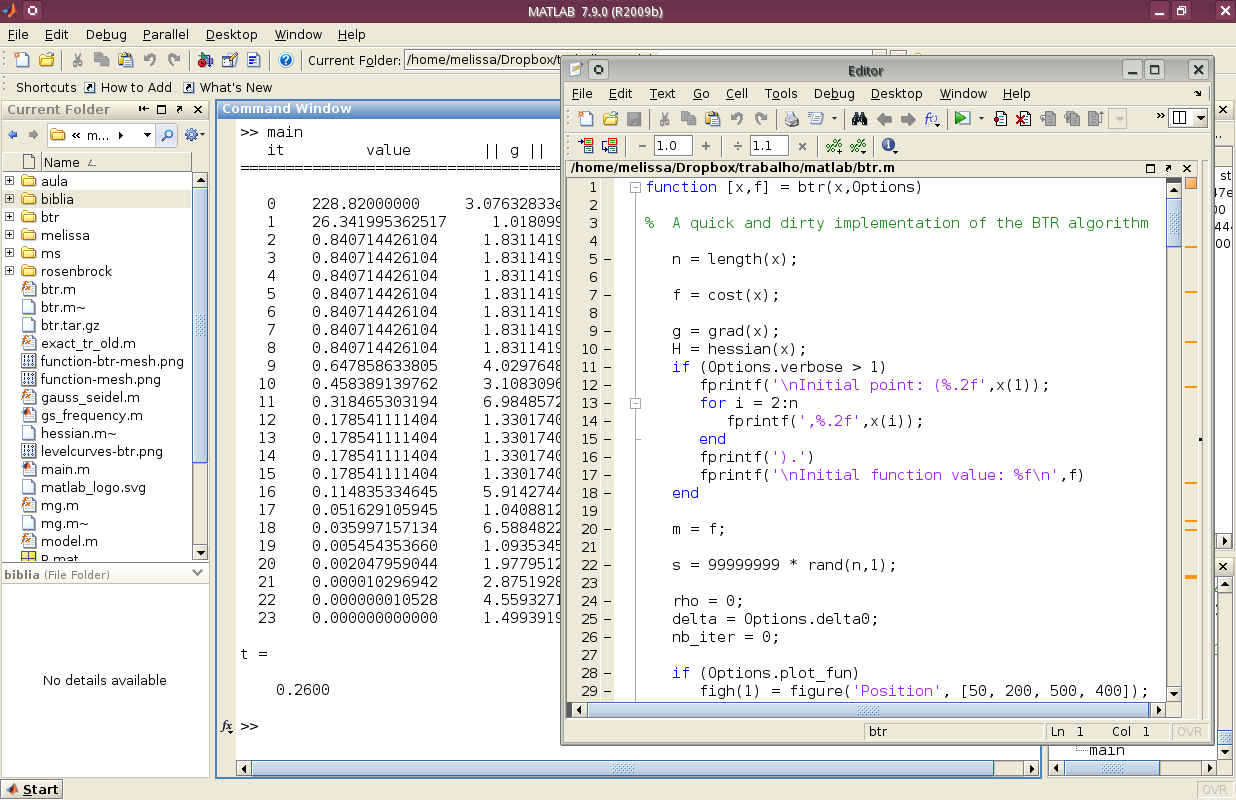
\includegraphics[width=8cm]{img/matlab.png}
   \end{center}
\end{frame}
\begin{frame}
   \frametitle{Exemplo de código em MATLAB}
   \begin{center}
	\begin{itemize}
		\item[] function[abs] = modulo(a)
		\item[]
		\begin{itemize}
			\item[] if $a > 0$
			\begin{itemize}
				\item[] modulo$=a$
		   \end{itemize}
		   \item[] else
		   \begin{itemize}
				\item[] modulo$=-a$
		   \end{itemize}
		   \item[] end
		\end{itemize}
	\end{itemize}
	\end{center}
\end{frame}
\begin{frame}
   \frametitle{Octave}
   Também um ambiente de programação, \emph{livre}, gratuito, que suporta a linguagem MATLAB.
   \begin{center}
      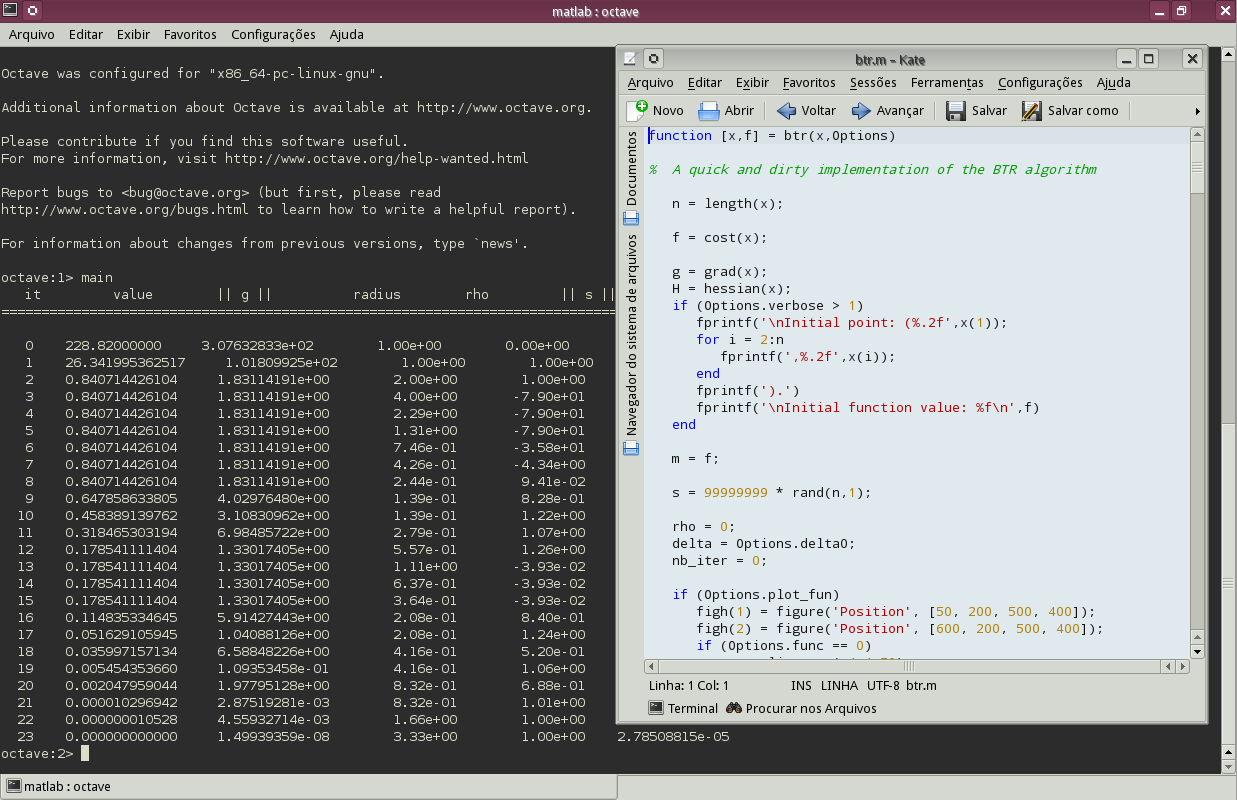
\includegraphics[width=8cm]{img/octave.png}
   \end{center}
\end{frame}

\end{document}
